\section{Renormalization of Wilson Lines}
In this section we will look at the renormalization properties of Wilson lines, and in particular find the cusp anomalous dimension. Later we will see that the cusp anomalous dimension appear in evolution equations for parton distributions and in the exponent of the exponentiated eikonal cross section. Hence, it is a fundamental ingredient in resummation with Wilson lines. 

There are two kinds of cusp anomalous dimensions, one is for Wilson lines on light-cone and one for Wilson lines off light-cone. We are considering the case of massless quarks, so the Wilson lines on light-cone is those of main focus, i.e. we need the on light-cone cusp anomalous dimension. We will show one way of calculating it in the next section, but first we will show how it appears.


In order to find the behaviour of Wilson lines at different scales, we can use the basic principle that the bare definition must be independent on the renormalization scale, i.e. the bare Wilson line satifies
\begin{align}\label{eq:bare wilson line}
    \mu\dv{}{\mu}\mathcal{U}_{\gamma}^{0}=0\,.
\end{align}
The bare Wilson line is given in terms of the bare coupling $g_0$ and the bare gauge field. Let us then rescale the field as in \cref{eq:rescaled gauge field QCD}, and use \cref{eq:counterterms} to define the relation
\begin{align}
    \mathcal{Z}_{3}^{1/2}g_{0}=\mathcal{Z}_{g}g\,,
\end{align}
giving the renormalized Wilson line\footnote{The scale factor $\mu$ is as usual hidden in g, i.e. we always make the substitution $g(\mu)\rightarrow\mu^{d-4}g$.}
\begin{align}
    \mathcal{U}_{\gamma}(g,\mu)=\mathcal{P}\exp{ig\mathcal{Z}_{g}\int_{\gamma}dz^{\mu}A_{\mu}(z)}\,.
\end{align}
A smooth Wilson with no cusps is completely renormalized as long as the coupling and the field is renormalized \cite{POLYAKOV1980171,DOTSENKO1980527}. Hence, by applying \cref{eq:bare wilson line} we would find a regular Callan-Symanzik equation. 

However, since we are studying a quark--antiquark pair that meets at a point and annihilates we are in interested in paths with cusps. These cusps will contribute with additional UV-divergences, so-called cusp divergences. A cusp in a Wilson line is characterized by two directional vectors $n_{1}^{\mu}$ and $n_{2}^{\mu}$ and the cusp divergence is a function of the angle $\chi$ between these two vectors. In Minkowski space this angle is defined as
\begin{align}\label{eq:Minkowski space angle}
    \cosh \chi=\frac{n_{1}\cdot n_2}{\sqrt{n_{1}^{2}n_{2}^{2}}}\,,
\end{align}
and the Wilson line will acquire a dependency on the regulator $\epsilon$ in dimensional regularization, i.e. $\mathcal{U}_{\gamma}(g,\mu,\epsilon)$. If both vectors are off light-cone, i.e. $n_{1}^{2}\neq 0$ and $n_{2}^{2}\neq 0$, the cusp divergences can be treated multiplicatively by introducing a multiplicative factor $\mathcal{Z}_{\text{cusp}}$ \cite{DOTSENKO1980527,Korchemsky:1987wg}
\begin{align}
    \widetilde{\mathcal{U}}_{\gamma}(g,\mu)=\mathcal{Z}_{\text{cusp}}(\chi,g,\mu,\epsilon)\,\mathcal{U}_{\gamma}(g,\mu,\epsilon)
\end{align}
giving the Callan-Symanzik equation
\begin{align}
    \Big(\mu\pdv{}{\mu}+\beta(g)\pdv{}{g}\Big)\,\ln\widetilde{\mathcal{U}}_{\gamma}(g,\mu)=\Gamma_{\text{cusp}}(\chi,g)\,,
\end{align}
where the cusp anomalous dimension is given by
\begin{align}
    \Gamma_{\text{cusp}}(\chi,g)=\lim_{\epsilon\to 0}\frac{\mu}{\mathcal{Z}_{\text{cusp}}}\dv{}{\mu}\mathcal{Z}_{\text{cusp}}(\chi,g,\epsilon)=\lim_{\epsilon\to 0}\dv{}{\ln\mu}\ln\mathcal{Z}_{\text{cusp}}(\chi,g,\epsilon)\,.
\end{align}
In regular UV-renormalization we have that the renormalization factor removes the $\epsilon$ dependence via counterterms, see \cref{sec:Renormalization}. Hence, we can calculate a Wilson line with cusps in perturbation theory and use $\mathcal{Z}_{\text{cusp}}$ to pull out the divergent part.  

If one or both vectors are on the light-cone, we can no longer use the multiplicative renormalization technique. This follows from the fact that for light-like vectors, \cref{eq:Minkowski space angle} blows up, and creates additional divergences. In dimensional regularization these additional divergences are double poles, i.e. of the form $1/\epsilon^{2}$. In \cref{sec:NLO drell yan calculation} we found that by adding the real and virtual gluon emission the double pole vanished and the cross section acquired large logarithmic dependancy. Thus, treating the $1/\epsilon
^{2}$ divergence would give a way of managing these large contributions by the renormalization properties of Wilson lines. 

Now, there is a relation between the on light-cone and off light-cone cusp anomalous dimension that we can use. In \cite{KORCHEMSKAYA1992169} it was found that the relation between the two in the limit of large $\chi$, is given by
\begin{align}\label{eq:off lightcone and on lightcone}
    \lim_{\chi\rightarrow\infty}\Gamma_{\text{cusp}}(\chi,g)=\chi\Gamma_{\text{cusp}}(g)+\mathcal{O}(\chi^{0})\,.
\end{align}
In this large limit, it follows from \cref{eq:Minkowski space angle} that
\begin{align}\label{eq:large minkowski limit}
    \chi=\ln\Big(\frac{2n_{1}\cdot n_{2}}{\sqrt{n_{1}^{2}n_{2}^{2}}}\Big)\,.
\end{align}
We observe that if we differentiate \cref{eq:off lightcone and on lightcone} with respect to $\ln n_{1}\cdot n_2$ we remove the troublesome denominator that blows up for light-like vectors. Therefore, we can write the on light-cone cusp anomalous dimension as\footnote{If the $\epsilon\rightarrow 0$ limit seem sketchy it is ment to be happen after the differentiation has been performed.}
\begin{align}\label{eq:on lightcone cusp anomalous}
    \Gamma_{\text{cusp}}(g)=\lim_{\epsilon\to 0}\dv{}{\ln n_1\cdot n_2}\dv{}{\ln\mu}\ln\mathcal{Z}_{\text{cusp}}(\chi,g,\epsilon)\,,
\end{align}
which is the expression we will use after we have calculated $\Gamma(\chi,g)$ in the next section.
%We can then integrate over $n_{1}\cdot n_2$, giving the modified Callan-Symanzik equation
%\begin{align}
%    \Big(\mu\pdv{}{\mu}+\beta(g)\pdv{}{g}\Big)\,\ln\widetilde{\mathcal{U}}_{\gamma}(g,\mu)=\Gamma_{\text{cusp}}(g)\ln n_{1}\cdot n_{2}+\Gamma(g)\,,
%\end{align}
%where $\Gamma(g)$ is some integration constant.

Wilson lines with endpoints will also have their own renormalization factors, and a corresponding endpoint anomalous dimension \cite{KORCHEMSKY1986459}. But we will only consider semi-infinite Wilson lines with endpoint at infinity. These contains IR-divergnces, which we will treat with an exponential regulator that suppress such contributions. 

\subsection{One-Loop Cusp Anomalous Dimension}
To calculate the one-loop cusp anomalous dimension, we consider the case of two semi-infinite Wilson lines bounded from below, see \cref{eq:semi-infinite Wilson line 0-to-infty}. We denote these as
\begin{align}
    \mathcal{U}_{\gamma_1}[\infty,0]&=\mathcal{P}\exp\Big(ig\int_{0}^{\infty}d\lambda_1\,n_{1}\cdot A(\lambda_1 n_1)\Big)\,,
    \\
    \mathcal{U}_{\gamma_2}[\infty,0]&=\mathcal{P}\exp\Big(ig\int_{0}^{\infty}d\lambda_2\,n_{2}\cdot A(\lambda_2 n_2)\Big)\,.
\end{align}

To construct the geometry of the diagrams in \cref{fig:one loop cusp anomalous dimension}, we use that Wilson lines are path-transitive and can be written as the composition\footnote{We could have used $\mathcal{W}_{DY}$ to calculate the cusp anomalous dimension, but that calculation is more complicated.}
\begin{align}\label{eq:wedged wilson line}
    \mathcal{U}_{\wedge}(0)=\mathcal{U}_{\gamma_1}[\infty,0]\mathcal{U}_{\gamma_2}[\infty,0]\,.
\end{align}
Expanding \cref{eq:wedged wilson line} to $\mathcal{O}(g^{2})$, we find
\begin{align}\label{eq:two wilson expansion}
    \mathcal{U}_{\wedge}(0)&=1+igt^{a}n_{1}^{\mu}\int_{0}^{\infty}d\lambda_1\,A_{\mu}^{a}(\lambda_{1}n_1)+igt^{b}n_{2}^{\mu}\int_{0}^{\infty}d\lambda_2\,A_{\mu}^{b}(\lambda_{2}n_2)\nonumber
    \\
    &\hspace{1cm}-g^{2}t^{a}t^{b}n_{1}^{\mu}n_{2}^{\nu}\int_{0}^{\infty}d\lambda_1\int_{0}^{\infty}d\lambda_2\,A_{\mu}^{a}(\lambda_1n_1)A_{\nu}^{b}(\lambda_2n_2)\,,
\end{align}
which follows from the expansions we discussed in \cref{sec:wilson line properties}. But in \cref{sec:wilson line properties} we integrated over $\lambda$ directly by Fourier transforming the fields, giving \cref{eq:semi-infinite Wilson line 0-to-infty}. In momentum space, we have IR-divergences when $n\cdot k\rightarrow 0$ and $k^{2}\rightarrow 0$. These originate from the Wilson line propagator and after the gauge fields have been Wick contracted to give the gauge field propagator. However, it is easier to work in coordinate space for this calculation. The IR-divergence in coordinate space originates from $\lambda\rightarrow\infty$, so to treat it we insert an exponential regulator in the exponent of the Wilson lines
\begin{fmffile}{wilsonone}
\begin{figure}
\centering
\begin{fmfgraph*}(150,100)
\fmfleft{i1} 
\fmfright{o1,o2}
\fmf{fermion}{i1,v1}
\fmf{fermion}{i1,v2}
\fmf{plain}{v1,o1}
\fmf{plain}{v2,o2}
\fmflabel{$\lambda_1 n_1$}{v2}
\fmflabel{$\lambda_2 n_2$}{v1}
\fmffreeze
\fmf{gluon}{v1,v2}
\end{fmfgraph*}
\hspace{1cm}
\begin{fmfgraph*}(150,100)
\fmfleft{i1} 
\fmfright{o1,o2}
\fmf{fermion}{i1,o1}
\fmf{plain,label=$\lambda_{1}n$,l.side=left}{i1,v2}
\fmf{fermion}{v2,v3}
\fmf{plain, label=$\lambda_2 n$,l.side=left}{v3,o2}
\fmffreeze
\fmf{gluon,left,tension=0}{v2,v3}
\end{fmfgraph*}
\caption{Wilson line diagrams contributing to the one-loop cusp anomalous dimension $\Gamma(\chi,g)$.}
\label{fig:one loop cusp anomalous dimension}
\end{figure}
\end{fmffile}
%%%%%%%%%%%%%%
\begin{align}\label{eq:IR regularized Wilson line}
    \mathcal{U}^{\delta}[\infty,0]=\mathcal{P}\exp(ig\int_{0}^{\infty}d\lambda\,n\cdot A(\lambda n)e^{-\delta\lambda\sqrt{-n^{2}}})\,,
\end{align}
which was proposed for Wilson line calculations in \cite{article}. The idea here is that $\delta\sqrt{-n^{2}}>0$, so that the exponential factor smoothly cuts off the $\lambda\rightarrow\infty$ contribution. This is guaranteed to yield an IR-finite result for the integral in \cref{eq:IR regularized Wilson line}, and all the remaining poles are of UV origin, i.e. $\lambda\rightarrow 0$.  

\subsubsection*{One-Loop Calculation}
To calculate the full cusp anomalous dimension $\Gamma_{\text{cusp}}(\chi,g)$, we would have to calculate both diagrams in \cref{fig:one loop cusp anomalous dimension}. But as we can see, the diagram on the right-hand does not depend on the cusp angle as the radiation is from the same line, so to find $\Gamma_{\text{cusp}}(g)$ we only focus on the left-hand diagram. 

To calculate this contribution we consider the expectation value
\begin{align}\label{eq:wedge wilson loop}
    \mathcal{W}_{\wedge}=\bra{0}\mathcal{T}\mathcal{U}_{\wedge}(0)\ket{0}\,
\end{align}
where the $\mathcal{T}$ is the time-ordering operator. Expanding \cref{eq:wedge wilson loop} to $\mathcal{O}(g^{2})$ using the expansion in \cref{eq:two wilson expansion}, will give
\begin{align}
    \mathcal{W}_{\wedge}&=1+\mathcal{W}_{\wedge}^{(1)}\nonumber
    \\
    &=1-g^{2}t^{a}t^{b}n_{1}^{\mu} n_{2}^{\mu}\int_{0}^{\infty}d\lambda_{1}\int_{0}^{\infty}d\lambda_{2}\,D_{\mu\nu}^{ab}(\lambda_{1}n_1-\lambda_{2}n_2)\,,
\end{align}
where we Wick contracted the emitted gluons to give the propagator. The propagator in coordinate space is given by \cite{article},
\begin{align}
    D_{\mu\nu}^{ab}(x-y)=-\mathcal{N}\frac{g_{\mu\nu}\delta^{ab}}{(-(x-y)^{2}+i\epsilon)^{d/2-1}}\,,
\end{align}
where
\begin{align}
    \mathcal{N}=\frac{\Gamma(d/2-1)}{4\pi^{d/2}}\,.
\end{align}
Here we should keep in mind that the Feynman prescription $i\epsilon$ and the regulator $\epsilon$ are not the same when we expand in $d=4-2\epsilon$. 

Let us then insert the IR-regulator given in \cref{eq:IR regularized Wilson line}, giving the expression
\begin{align}\label{eq:amplitude radiation wilson line cusp}
    \mathcal{W}_{\wedge}^{(1)}&=-g^{2}t^{a}t^{b}n_{1}^{\mu} n_{2}^{\mu}\int_{0}^{\infty}d\lambda_{1}\int_{0}^{\infty}d\lambda_{2}\,D_{\mu\nu}^{ab}(\lambda_{1}n_1-\lambda_{2}n_2)\,e^{-\delta(\lambda_1\sqrt{-n_{1}^{2}}+\lambda_2\sqrt{-n_{2}^{2}})}\nonumber
    \\
    &=g^{2}C_{F}\mathcal{N}(\epsilon)n_{1}\cdot n_{2}\int_{0}^{\infty}d\lambda_{1}\int_{0}^{\infty}d\lambda_{2}\,\frac{e^{-\delta(\lambda_1\sqrt{-n_{1}^{2}}+\lambda_2\sqrt{-n_{}^{2}})}}{(-(\lambda_{1}n_{1}-\lambda_{2}n_{2})^{2})^{1-\epsilon}}\,.
\end{align}
To evaluate the integrals we can make the change of variables
\begin{align}
    \lambda_1&=\frac{\alpha x}{\sqrt{-n_{1}^{2}}}\,,
    \\
    \lambda_{2}&=\frac{\alpha(1-x)}{\sqrt{-n_{2}^{2}}}\,,
\end{align}
where $x\in[0,1]$ and $\alpha\in[0,\infty)$, giving the Jacobian
\begin{align}
    \mathcal{J}=\frac{\alpha}{\sqrt{n_{1}^{2}n_{2}^{2}}}\,.
\end{align}
With these changes we get the following integral
\begin{align}
    I&=\int_{0}^{\infty}d\lambda_{1}\int_{0}^{\infty}d\lambda_{2}\,\frac{e^{-\delta(\lambda_1\sqrt{-n_{1}^{2}}+\lambda_2\sqrt{-n_{}^{2}})}}{(-(\lambda_{1}n_{1}-\lambda_{2}n_{2})^{2})^{1-\epsilon}}\nonumber
    \\
    &=\frac{1}{\sqrt{n_{1}^{2}n_{2}^{2}}}\int_{0}^{1}dx \frac{1}{(x^{2}+(1-x)^{2}+2x(1-x)\cosh\gamma)^{1-\epsilon}}\int_{0}^{\infty}d\alpha\,e^{-\delta\alpha}\alpha^{-1+2\epsilon}\,,
\end{align}
where we defined 
\begin{align}\label{eq:gamma minkowski}
    \cosh\gamma=-\frac{n_{1}\cdot n_{2}}{\sqrt{n_{1}^{2}n_{2}^{2}}}\,,
\end{align}
and by inserting this back into \cref{eq:amplitude radiation wilson line cusp}, we get
\begin{align}
    \mathcal{W}_{\wedge}^{(1)}=-g^{2}C_{F}\mathcal{N}(\epsilon)\int_{0}^{1}dx\frac{\cosh\gamma}{(x^{2}+(1-x)^{2}+2x(1-x)\cosh\gamma)^{1-\epsilon}}\int_{0}^{\infty}d\alpha\,e^{-\delta\alpha}\alpha^{-1+2\epsilon}\,.
\end{align}

Let us evaluate the $\alpha$ integral by another change of variable $y=\alpha\delta$, giving
\begin{align}
    \int_{0}^{\infty}d\alpha\,e^{-\delta\alpha}\alpha^{-1+2\epsilon}=\delta^{-2\epsilon}\int_{0}^{\infty}dy\,e^{-y}y^{-1+2\epsilon}=\delta^{-2\epsilon}\,\Gamma(2\epsilon)\,,
\end{align}
where we used the integral representation of the Gamma function. This gamma function has the expansion as $\epsilon\rightarrow 0$
\begin{align}
    \Gamma(2\epsilon)=\frac{1}{2\epsilon}+\mathcal{O}(\epsilon^{0})\,.
\end{align}

The $x$ integral can be rewritten in terms of the hypergeometric function $_{2}F_{1}$. However, we want the expansion in the limit $\epsilon\rightarrow 0$, so it is inconvenient to use this representation. Let us instead set $\epsilon=0$ in this integral, giving
\begin{align}
    \int_{0}^{1}dx\frac{\cosh\gamma}{(x^{2}+(1-x)^{2}+2x(1-x)\cosh\gamma)}=\gamma\coth\gamma\,.
\end{align}
This integral would not be convergent without the definition of $\gamma$ in \cref{eq:gamma minkowski}. But we want our result in terms of $\chi$, and from \cref{eq:Minkowski space angle} these are related in the following way
\begin{align}
    \cosh\gamma&=-\cosh\chi=\cosh(\chi+i\pi)\,,
\end{align}
giving
\begin{align}
    \gamma=\chi+i\pi
\end{align}
and
\begin{align}
    \coth(\chi+i\pi)=\coth\chi\,.
\end{align}
Also, we can safely neglect the terms that are non singular for $\epsilon\rightarrow 0$, i.e. $\delta^{-2\epsilon}\rightarrow 1$ and $\mathcal{N}(\epsilon)\rightarrow 1/4\pi^{2}$. This removes the IR regulator $\delta$ from the expression in a smooth way. Using all these relations, we find that the $\mathcal{O}(g^{2})$ expansion of the Wilson loop expectation value takes the form
\begin{align}\label{eq:one loop wedge wilson loop}
    \mathcal{W}_{\wedge}^{(1)}&=-g^{2}\,C_{F}\,\mathcal{N}(\epsilon)\,\delta^{-2\epsilon}\,\Gamma(2\epsilon)\,\gamma\coth\gamma\nonumber
    \\
    &=-g^{2}\,C_{F}\,\frac{1}{4\pi^{2}}\,\frac{1}{2\epsilon}\,(\chi+i\pi)\coth\chi\,.
\end{align}
As mentioned above, this is only one contribution to the cusp anomalous dimension $\Gamma_{cusp}(\chi,g)$. But the other contribution does not depend on the cusp angle, so when we perform the differentiation with respect to $\ln n_1\cdot n_2$ it will not contribute to $\Gamma_{cusp}(g)$ that we are interested in.

\subsubsection*{Cusp Anomalous Dimension $\Gamma_{\text{cusp}}(g)$}
In \cref{eq:on lightcone cusp anomalous} we had that the cusp anomalous dimension for Wilson lines on light-cone could be written as
\begin{align}
    \Gamma_{\text{cusp}}(g)=\lim_{\epsilon\to 0}\dv{}{\ln n_1\cdot n_2}\dv{}{\ln\mu}\ln\mathcal{Z}_{\text{cusp}}(\chi,g,\epsilon)\,.
\end{align}
To find $\Gamma_{\text{cusp}}(g)$ we can now use that $\mathcal{Z}_{\text{cusp}}$ is used to cancel the $\epsilon$ divergence from the Wilson line in \cref{eq:one loop wedge wilson loop}. We can also introduce the dependence on the scale $\mu$ in the usual way $g^{2}\rightarrow \mu^{2\epsilon}g^{2}$, giving the cusp factor 
\begin{align}
    \mathcal{Z}_{\text{cusp}}=1+g^{2}\mu^{2\epsilon}C_{F}\frac{1}{4\pi^{2}}\frac{1}{2\epsilon}(\chi+i\pi)\coth\chi\,.
\end{align}
Performing the differentiation and keeping only terms to $\mathcal{O}(g^{2})$, we find
\begin{align}
    \Gamma_{\text{cusp}}(g)&=\lim_{\epsilon\to 0}\dv{}{\ln n_1\cdot n_2}\mu\dv{}{\mu}\ln\Big(1+g^{2}\mu^{2\epsilon}C_{F}\frac{1}{4\pi^{2}}\frac{1}{2\epsilon}(\chi+i\pi)\coth\chi\Big)\nonumber
    \\
    &=\dv{}{\ln n_1\cdot n_2}\Big(g^{2}C_{F}\frac{1}{4\pi^{2}}(\chi+i\pi)\coth\chi\Big)\nonumber
    \\
    &=\frac{g^{2}}{4\pi^{2}}C_{F}\,,
\end{align}
where we in the last differentiation used that $\chi$ is given by \cref{eq:large minkowski limit} in the large limit, and that $\coth\chi=1$ in this limit. At first sight the this might seem a little fishy as the derivative of the logarithm gives the argument in the denominator. But if we expand this denominator it will give a $\mathcal{O}(g^{4})$ term and we are only considering the $\mathcal{O}(g^{2})$ correction. As usual we use that $\alpha_s=g^{2}/4\pi$, giving
\begin{align}\label{eq:one-loop cusp anomalous dimension}
    \Gamma_{\text{cusp}}(\alpha_s)=\frac{\alpha_s}{\pi}C_{F}\,,
\end{align}
which is the well known one-loop cusp anomalous dimension for a Wilson line in the fundamental representation \cite{Korchemsky:1987wg}.  


\section{Exponentiation of Parton-In-Parton Distributions}\label{sec:RGE for parton in parton}
In \cref{sec:QCD and Collinear factorization}, we discussed the renormalization group equation for the parton distribution functions $f_{i/P}(x,\mu)$, i.e. the DGLAP equation. Now we would like to discuss the renormalization group equations for the parton-in-parton disttribution functions $f_{i/i}$. In \cref{sec:lightcone parton in parton distributions} we derived the parton-in-parton distributions, given by
\begin{align}
    f_{i/i}(x)=\int\frac{dy^{-}}{4\pi}e^{-ixp^{+}y^{-}}\bra{q}\overline{\Psi}(y^{-})\gamma^{+}\Psi(0)\ket{q}\,,
\end{align}
where the product in the matrix element are eikonal fermions\footnote{Or particles dressed with Wilson lines.}. In \cite{Korchemsky:1988si} it was found that in the limit $x\rightarrow 1$, the parton-in-parton distributions obeys the evolution equation
\begin{align}\label{eq:RGE partoninparton}
    \mu\dv{}{\mu}f_{i/i}(x,\mu)=\int_{x}^{1}\frac{dz}{z}P_{i/i}\big(\frac{x}{z},\alpha_s\big)f_{i/i}(z,\mu)+\mathcal{O}((1-x)^{0})\,,
\end{align}
where the splitting functions has the asymptotic behaviour 
\begin{align}\label{eq:asymptotic splitting function}
    P_{i/i}(z,\alpha_s)=2\Gamma_{\text{cusp}}^{(i)}(\alpha_s)\Big[\frac{1}{1-z}\Big]_{+}+2C^{(i)}(\alpha_s)\delta(1-z)+\mathcal{O}((1-z)^{0})\,,
\end{align}
which is true to all order \cite{Korchemsky:1988si}, and the one-loop $\Gamma_{\text{cusp}}^{(q,\bar{q})}$ is the one we found in \cref{eq:one-loop cusp anomalous dimension}. We can verify this behaviour by taking the limit $z\rightarrow 1$ of the splitting functions we found in \cref{eq:qq splitting function} and \cref{eq:gg splitting function}, giving
\begin{align}
    P_{q/q}(z)&=2C_{F}\frac{\alpha_s}{\pi}\Big(\Big[\frac{1}{1-z}\Big]_{+}+\frac{3}{4}\delta(1-z)\Big)+\mathcal{O}(\alpha_{s}^{2})\,,
    \\
    P_{g/g}(z)&=2\frac{\alpha_s}{\pi}\Big(C_{A}\Big[\frac{1}{1-z}\Big]_{+}+\frac{\beta_{0}}{4}\delta(1-z)\Big)+\mathcal{O}(\alpha_{s}^{2})\,,
\end{align}
where $\beta_0$ is the one-loop beta coefficient, see \cref{eq:beta one-loop}, and we observe that the cusp anomalous dimension for $q,\bar{q}$ corresponds to the one we found in \cref{eq:one-loop cusp anomalous dimension}. We also observe that the cusp anomalous dimension for $i=g$ is given by
\begin{align}
    \Gamma_{\text{cusp}}^{(g)}(\alpha_s)=\frac{\alpha_s}{\pi}C_{A}+\mathcal{O}(\alpha_{s}^{2})\,,
\end{align}
which is just a matter of making the calculation we did in \cref{eq:one-loop cusp anomalous dimension} by using Wilson lines in the adjoint representation giving the Casimir invariant $C_{A}$. We can also read of the one-loop expression for $C^{(i)}$, given by
\begin{align}
    C^{(q,\bar{q})}(\alpha_s)&=\frac{\alpha_s}{\pi}\frac{3}{4}C_{F}+\mathcal{O}(\alpha_{s}^{2})\,,\label{eq:C for quarks}
    \\
    C^{(g)}(\alpha_s)&=\frac{\alpha_s}{\pi}\frac{\beta_{0}}{4}+\mathcal{O}(\alpha_{s}^{2})\,,\label{eq:C for gluons}
\end{align}

In order to solve \cref{eq:RGE partoninparton} we take the Mellin transform, giving the large $N$ equation\footnote{Remember that $z\rightarrow 1$ corresponds to to large N.}
\begin{align}
    \mu\dv{}{\mu}f_{i/i}(N,\mu)=P_{i/i}(N,\alpha_{s})f_{i/i}(N,\mu)+\mathcal{O}(1/N)\,.
\end{align}
where the moments of the splitting function takes the form
\begin{align}
    P_{i/i}(N,\alpha_s)&=2\Gamma_{\text{cusp}}^{(i)}(\alpha_s)\int_{0}^{1}dz\,z^{N-1}\Big[\frac{1}{(1-z)_{+}}\Big]+2C^{(i)}(\alpha_s)\int_{0}^{1}dz\,z^{N-1}\delta(1-z)\nonumber
    \\
    &=-2\Gamma_{\text{cusp}}^{(i)}(\alpha_s)\ln\bar{N}+2C^{(i)}(\alpha_s)\,,
\end{align}
where we neglect constant terms from the Mellin transform, see \cref{eq:App mellin of ln plus dist}. These constant terms would reproduce the constant terms we neglected in \cref{eq:Mellin space NLO of omegaqbarq}, so we do the same here. Hence, the evolution equation in Mellin space take the form
\begin{align}
    \dv{}{\ln\mu}\ln f_{i/i}(N,\mu)=-2\Gamma_{\text{cusp}}^{(i)}\ln\bar{N}+2C^{(i)}(\alpha_s)\,.
\end{align}
with the solution
\begin{align}\label{eq:RGE parton in parton}
    f_{i/i}(N,\mu)=\exp{-\int_{0}^{\mu^{2}}\frac{d\mu'^{2}}{\mu'^{2}}\Big(\Gamma_{\text{cusp}}^{(i)}(\alpha_{s}(\mu'))\ln\bar{N}-C^{(i)}(\alpha_{s}(\mu'))\Big)}\,.
\end{align}
where we have chosen the initial condition $f_{i/i}(N,\mu=0)=1$.

For the eikonal distributions $f_{i/i}^{(\text{eik})}$ there is a slight modification. We want them to be sum of plus distributions, so from \cref{eq:asymptotic splitting function} we must have that $C^{i}=0$. The solution can then be written as
\begin{align}\label{eq:RGE parton in parton eikonal}
    f_{i/i}^{(\text{eik})}=\exp{-\int_{0}^{\mu^{2}}\frac{d\mu'^{2}}{\mu'^{2}}\Gamma_{\text{cusp}}^{(i)}(\alpha_{s}(\mu')\ln\bar{N}}\,.
\end{align}
Notice that the choice of the lower boundary diverges for $\mu\rightarrow 0$, which will be used later to cancel divergences coming from $\Me{\sigma}^{\text{(eik)}}(N,\epsilon)$. The equations for $J_{i/i}$ and $J_{i/i}^{(\text{eik})}$ are completely analogous. 

\subsection{Hard Virtual Gluons}
With the solutions in \cref{eq:RGE parton in parton} and \cref{eq:RGE parton in parton eikonal} we are now ready to compute the ratios of distributions we had in \cref{eq:partonic and eikonal plus ration}. But first, we mentioned in \cref{sec:factorization soft gluons} that the main difference between the partonic function $\omega_{ij}$ and its eikonal approximation $\omega_{ij}^{(\text{eik})}$ are contributions $G_{ij}(Q,\mu)$ from hard virtual gluons \cite{KORCHEMSKY1993433}. So in general, we can write the relation between the two as
\begin{align}\label{eq:relation w and eikonal w}
    \Me{\omega}_{ij}(N,Q,\mu,\alpha_{s}(\mu))=H_{ij}(Q,\alpha_{s}(\mu))\,G_{ij}(Q,\mu)\,\Me{\omega}_{ij}^{(\text{eik})}(N,Q,\mu,\alpha_s)\,,
\end{align}
where $H(Q)$ is the same hard process without large logarithms. If we compare this expression with \cref{eq:partonic and eikonal plus ration}, we find that the hard virtual contributions are entirely describes by the ratios 
\begin{align}\label{eq:hard virtual gluons}
    G_{ij}(Q,\mu)=\Big[\frac{\Me{J}_{i/i}(N,Q,\epsilon)\Me{J}_{j/j}(N,Q,\epsilon)}{\tilde{f}_{i/i}(N,\mu,\epsilon)\tilde{f}_{j/j}(N,\mu,\epsilon)}\Big]\Big[\frac{\Me{f}_{i/i}^{(\text{eik})}(N,\mu,\epsilon)\,\Me{f}_{j/j}^{(\text{eik})}(N,\mu,\epsilon)}{\Me{J}_{i/i}^{(\text{eik})}(N,Q,\epsilon)\,\Me{J}_{j/j}^{(\text{eik})}(N,Q,\epsilon)}\Big]\,,
\end{align}
and as mentioned in \cref{sec:factorization soft gluons}, the two ratios are free of collinear divergences and so is $G(Q,\mu)$.  We can now use the solutions in \cref{eq:RGE parton in parton} and \cref{eq:RGE parton in parton eikonal} to compute the ratios, giving
\begin{align}\label{eq:ratio pdf and eikonal pdf}
    \frac{\Me{f}_{i/i}^{(\text{eik})}(N,\mu,\epsilon)\,\Me{f}_{j/j}^{(\text{eik})}(N,\mu,\epsilon)}{\tilde{f}_{i/i}(N,\mu,\epsilon)\tilde{f}_{j/j}(N,\mu,\epsilon)}=\exp{-2\int_{0}^{\mu^{2}}\frac{d\mu'^{2}}{\mu'^{2}}C^{(i)}(\alpha_{s}(\mu'))}\,,
\end{align}
where the logarithm $\ln\bar{N}$ accompanied by the cusp anomalous dimension has canceled. We have also used that $C^{(i)}=C^{(j)}$ for $i=q$ and $j=\bar{q}$, giving two times $C^{(i)}$\footnote{We choose to use generic subscripts even if we really mean $i=q$. In this way it would be easier to generalize to cases where we also have $i=g$.}. The ratio of jet distributions are equivalent, with the difference of $Q$ instead of $\mu$, i.e.
\begin{align}\label{eq:ratio jets and eikonal jets}
    \frac{\Me{J}_{i/i}(N,Q,\epsilon)\Me{J}_{j/j}(N,Q,\epsilon)}{\Me{J}_{i/i}^{(\text{eik})}(N,Q,\epsilon)\,\Me{J}_{j/j}^{(\text{eik})}(N,Q,\epsilon)}=\exp{2\int_{0}^{Q^{2}}\frac{d\mu'^{2}}{\mu'^{2}}C^{(i)}(\alpha_{s}(\mu'))}\,.
\end{align}
If we insert \cref{eq:ratio pdf and eikonal pdf} and \cref{eq:ratio jets and eikonal jets} into \cref{eq:hard virtual gluons}, we get after reshuffling the ratios that the contribution from hard virtual gluons can be written as
\begin{align}
    G_{ij}(Q,\mu)=\exp{2\int_{\mu^{2}}^{Q^{2}}\frac{d\mu'^{2}}{\mu'^{2}}C^{(i)}(\alpha_{s}(\mu'))}\,,
\end{align}
where we observe that by choosing $Q$ as an argument in the jet distributions, we have a contribution from this expression. But we have already set $Q=\mu$ on several occasions, so for the simplified result we do the same here, giving that $G_{ij}(Q,Q)=1$. With this choice we have from \cref{eq:relation w and eikonal w} that the partonic function $\Me{\omega}_{ij}$ is given by
\begin{align}\label{eq:partonic and eikonal relation}
    \Me{\omega}_{ij}(N,Q,\mu,\alpha_{s}(\mu))=H_{ij}(Q,\alpha_{s}(\mu))\,\Me{\omega}_{ij}^{(\text{eik})}(N,Q,\mu,\alpha_{\mu})\,.
\end{align}

We have reduced the problem of resumming large logarithmic contributions to finding the eikonal function $\Me{\omega}_{ij}^{(\text{eik})}(N)$. Hence, we will in the next section turn our attention back to the eikonal cross section $\Me{\sigma}_{ij}^{\text{eik}}$ and how to calculate it. 

%%%%%%%%% Eikonal cross section %%%%%%%%%%%%%%%%%
\section{The Eikonal Cross Section}
In order to calculate the eikonal cross section $\Me{\sigma}_{ij}^{\text{eik}}$, we look at the Wilson loop expectation value $\mathcal{W}_{DY}$ we found in \cref{sec:factorization soft gluons}. We will first make an $\mathcal{O}(g^{2})$ expansion of the expectation value, and then use the non-Abelian eikonal exponentiation theorem to find the exponentiated form. Then we will use the factorized form of the eikonal cross section in \cref{eq:eikonal approcximation of partonic} to find $\Me{\omega}_{ij}
^{\text{(eik)}}$. 

So let us start from the expectation value
\begin{align}
    \mathcal{W}_{DY}(y)&=\bra{0}\Bar{T}\,\mathcal{U}_{DY}^{\dagger}(y)T\,\mathcal{U}_{DY}(0)\ket{0}\,,
\end{align}
where a one-loop contribution is illustrated in \cref{fig:DYwilsonloopcutpropagator}. By
using the momentum space expansion of Wilson lines derived in \cref{sec:wilson line properties}, we find that to $\mathcal{O}(g^{2})$
\begin{align}\label{eq:order g2 DY wilson loop}
    \mathcal{W}_{DY}=1+g^{2}C_{F}\int\frac{d^{d}k}{(2\pi)^{d}}2\pi\delta^{+}(k^{2})\frac{p_{1}\cdot p_{2}}{p_1\cdot k\,p_2\cdot k}(e^{-iy^{0}k^{0}}-1)\,,
\end{align}
where we have used that $p_{1}^{2}=p_{2}^{2}=0$. We have also used that in diagrams such as \cref{fig:DYwilsonloopcutpropagator}, we have to use a cut gluon propagator \cite{Korchemsky:1992xv}
\begin{align}
    D_{\mu\nu\,+}^{ab}(k)=-\delta^{ab}g_{\mu\nu}2\pi\delta^{+}(k^{2})\,.
\end{align}
To rewrite this further, we can use that the ratio of momenta is invariant under rescaling of $p_1$ and $p_2$. With light-cone coordinates (see \cref{sec:Appendix Light-cone coordinates}), we have that
\begin{align}
    \frac{p_{1}\cdot p_{2}}{p_1\cdot k\,p_2\cdot k}&=\frac{n_{1}\cdot n_{2}}{n_{1}\cdot k\,n_{2}\cdot k}=\frac{1}{k^{+}k^{-}}\label{eq:k+k- relation in calculation}
    \\
    k^{2}&=2k^{+}k^{-}-k_{\perp}^{2}
    \\
    k^{0}&=(k^{+}+k^{-})/\sqrt{2}\label{eq:energy relation lightcone momenta}
\end{align}
where we used that $n_1$ and $n_2$ are light-like vectors. Let us also use the measure $d^{d}k=dk^{+}dk^{-}d^{d-2}k_{\perp}$, such that with the above rewritings the expansion can be rewritten as
\begin{align}\label{eq:W(Drell) to one-loop}
    \mathcal{W}_{DY}&=1+\frac{\alpha_{s}}{\pi}C_{F}\int\frac{d^{d-2}k_{\perp}}{(2\pi)^{d-2}}\int dk^{+}dk^{-}\,2\pi\delta(2k^{+}k^{-}-k_{\perp}^{2})\frac{(e^{-iy^{0}(k^{+}+k^{-})/\sqrt{2}}-1)}{k^{+}k^{-}}\,,
\end{align}
where we pulled out a factor of $(2\pi)^{2}$ to give the coupling. On this form, it is not obvious how to treat these integrals as the limits on the $k^{+}$ and $k^{-}$ are unspecified. Instead we use the non-Abelian exponentiation theorem, where there are restrictions on the form of the exponent to preserve the exponentiation conditions.
%%%%%%%%%%%%%%% figure %%%%%%%%%%%%%%%
\begin{figure}
    \centering
    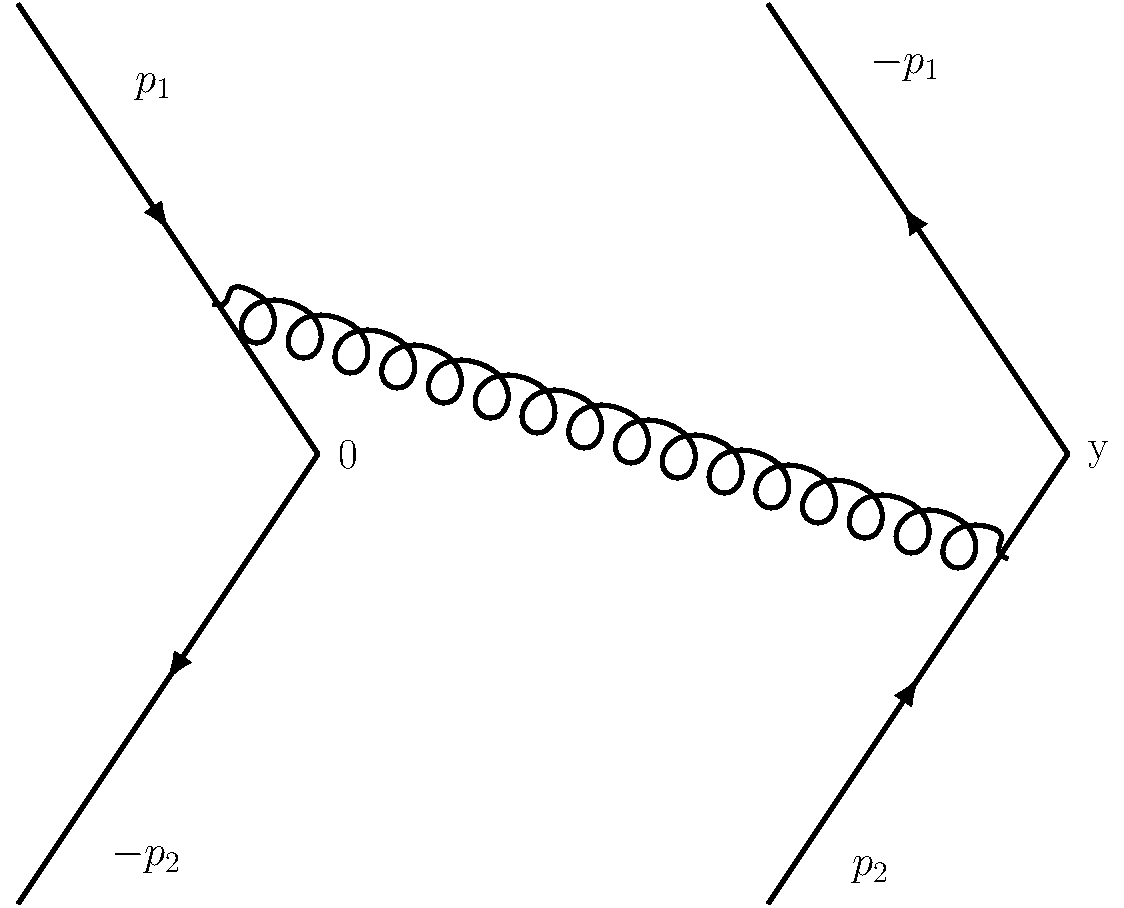
\includegraphics[scale=0.3]{Figures/DrellYanLoop.pdf}
    \caption{A one-loop contribution to the Drell-Yan eikonal cross section.}
    \label{fig:DYwilsonloopcutpropagator}
\end{figure}
%%%%%%%%%%%%%%%%%%%%%%%%%%%%%%%%%%%%%%
But before we give the procedure to find the eikonal cross section, we take a look at the structure of the expansion in \cref{eq:W(Drell) to one-loop}. We observe that the factor in front of the integral looks very much like the one-loop cusp anomalous dimension in \cref{eq:one-loop cusp anomalous dimension}. So if we use that the scale of the coupling is $\alpha_{s}(k_{\perp})$, we can write the expansion as\footnote{It is understood that it is the cusp anomalous dimension for particles in the fundamental representation.}
\begin{align}\label{eq:W(Drell) to one-loop number two}
    \mathcal{W}_{DY}&=1+\int\frac{d^{2-2\epsilon}k_{\perp}}{(2\pi)^{1-2\epsilon}}\Gamma_{\text{cusp}}(\alpha_{s}(k_{\perp}))\int dk^{+}dk^{-}\,\delta(2k^{+}k^{-}-k_{\perp}^{2})\frac{(e^{-iy^{0}(k^{+}+k^{-})/\sqrt{2}}-1)}{k^{+}k^{-}}\,,
\end{align}
where we have inserted for $d=4-2\epsilon$ and it is understood that one has to use the running coupling at one-loop order, e.g. the one-loop in \cref{eq:one-loop strong coupling}. Further, by using the non-Abelian exponentiation theorem we can write $\mathcal{W}_{DY}$ as
\begin{align}\label{eq:relation wDY and WDY}
    \mathcal{W}_{DY}=1+\sum_{n=1}^{\infty}\mathcal{W}_{DY}^{(n)}=\exp\Big(\sum_{n=1}^{\infty}W_{DY}^{(n)}\Big)\,,
\end{align}
where $W_{DY}$ are the webs we alluded to in \cref{sec:exponentiation}\footnote{For more details on webs, see \cite{White:2015wha,article}.}. For Drell-Yan, we have that $\mathcal{W}_{DY}^{(1)}=W_{DY}^{(1)}$, which we will use for our calculation. This is not true in general, but we are only interested in the one-loop result.

From the non-Abelian eikonal exponentiation theorem, the Mellin transformed eikonal cross section can on the most general form be written as \cite{laenen2000power}\footnote{The expression in \cite{laenen2000power} is for joint resummation, i.e. threshold and low transverse momentum of the final state. We are only considering threshold resummation, so we adjust the expression to our purpose.}
\begin{align}\label{eq:general result of eikonal cross section}
    \Me{\sigma}_{ij}^{\text{(eik)}}(N,Q,\epsilon)=\exp\Big(&2\int\frac{d^{4-2\epsilon}k}{\Omega_{1-2\epsilon}}\,\theta\Big(\frac{Q}{\sqrt{2}}-k^{+}\Big)\theta\Big(\frac{Q}{\sqrt{2}}-k^{-}\Big)\nonumber
    \\
    &W_{DY}\big(k^{2},\frac{n_{1}\cdot k\,n_{2}\cdot k}{n_{1}\cdot n_2},\mu,\alpha_{s},\epsilon\big)\Big(e^{-Nk^{0}/Q}-1\Big)\Big)\nonumber
    \\
    &=\exp\big(\Me{E}^{\text{(eik)}}(N,\epsilon)\big)\,,
\end{align}
where $W_{DY}$ is the web, and the invariance under rescaling of the momentum is applied. The theta functions are used to cut off the $k^{+}$ and $k^{-}$ integrals such that they are UV-finite and resctricts the $k_{\perp}$ integral to have the maximum value of $Q^{2}$. Without this restriction, the exponentiation conditions would not be valid \cite{Laenen:2004pm}. The appearance of $N$ in the exponent can be understood from the taking the Mellin transform of \cref{eq:order g2 DY wilson loop}, using the saddle point approximation $y^{0}\approx -iN/Q$ as discussed in \cite{KORCHEMSKY1993433}. The angular factor can in $d$-dimension be found in \cref{eq:d-dimensional sphere area}. 

We can now use that $W_{DY}^{(1)}=\mathcal{W}_{DY}^{(1)}$, and use \cref{eq:W(Drell) to one-loop number two} to write the exponent as
\begin{align}
    \Me{E}^{\text{(eik)}}(N,Q,\epsilon)&=2\int\frac{d^{2-2\epsilon}k_{\perp}}{\Omega_{1-2\epsilon}}\Gamma_{\text{cusp}}(\alpha_{s}(k_{\perp}))\int dk^{+}dk^{-}\,\theta\Big(\frac{Q}{\sqrt{2}}-k^{+}\Big)\theta\Big(\frac{Q}{\sqrt{2}}-k^{-}\Big)\nonumber
    \\
    &\hspace{2cm}\times\delta(2k^{+}k^{-}-k_{\perp}^{2})\frac{1}{k^{+}k^{-}}\big(e^{-N(k^{+}+k^{-})/\sqrt{2}Q}-1\big)\nonumber
    \\
    &=4\int\frac{d^{2-2\epsilon}k_{\perp}}{\Omega_{1-2\epsilon}}\frac{\Gamma_{\text{cusp}}(\alpha_{s}(k_{\perp}))}{k_{\perp}^{2}}\int\frac{dk^{+}}{2k^{+}}\,\theta\Big(\frac{Q}{\sqrt{2}}-k^{+}\Big)\theta\Big(\frac{Q}{\sqrt{2}}-\frac{k_{\perp}^{2}}{2k^{+}}\Big)\nonumber
    \\
    &\hspace{2cm}\times\Big(e^{-N\big(k^{+}+\frac{k_{\perp}^{2}}{2k^{+}}\big)/\sqrt{2}Q}-1\Big)
\end{align}
where we have applied the delta function over $k^{-}$. Because of the theta functions, the lower and upper limits of the $k^{+}$ integral are finite. Hence, the exponent take the form 
\begin{align}
    \Me{E}^{\text{(eik)}}(N,Q,\epsilon)&=4\int\frac{d^{2-2\epsilon}k_{\perp}}{\Omega_{1-2\epsilon}}\frac{\Gamma_{\text{cusp}}(\alpha_{s}(k_{\perp}))}{k_{\perp}^{2}}\int_{k_{\perp}^{2}/\sqrt{2}Q}^{Q/\sqrt{2}}\frac{dk^{+}}{2k^{+}}\Big(e^{-N\big(k^{+}+\frac{k_{\perp}^{2}}{2k^{+}}\big)/\sqrt{2}Q}-1\Big)\,.
\end{align}


%To treat the $k^{+}$ and $k^{-}$ integrals we will instead of using \cref{eq:k+k- relation in calculation}, use that $k^{+}k^{-}=(k^{2}+k_{\perp}^{2})/2$ which follows from \cref{App.eq:light-cone momenta squared}. Then by a change of variable using \cref{eq:minus ligh-cone momenta} and \cref{eq:energy relation lightcone momenta}, the exponent can be written as
%\begin{align}
%    \Me{E}^{\text{(eik)}}(N,Q,\epsilon)&=2\int\frac{d^{2-2\epsilon}k_{\perp}}{\Omega_{1-2\epsilon}}\int dk^{2}\int\frac{dk^{+}}{2k^{+}}\theta\Big(\frac{Q}{\sqrt{2}}-k^{+}\Big)\theta\Big(\frac{Q}{\sqrt{2}}-\frac{k_{\perp}^{2}+k^{2}}{2k^{+}}\Big)\nonumber
%    \\
%    &\hspace{1cm}W_{ij}\big(k^{2},k^{2}+k_{\perp}^{2},\mu,\alpha_{s},\epsilon\big)\Big(e^{-N\big(k^{+}+\frac{k_{\perp}^{2}+k^{2}}{2k^{+}}\big)/\sqrt{2}Q}-1\Big)\nonumber
%    \\
%    &=2\int\frac{d^{2-2\epsilon}k_{\perp}}{\Omega_{1-2\epsilon}}\int_{0}^{Q^{2}-k_{\perp}^{2}} dk^{2}\,W_{ij}\big(k^{2},k^{2}+k_{\perp}^{2},\mu,\alpha_{s},\epsilon\big)\nonumber
%    \\
%    &\hspace{0.5cm}\int_{(k_{\perp}^{2}+k^{2})/\sqrt{2}Q}^{Q/\sqrt{2}}\frac{dk^{+}}{2k^{+}}\Big(e^{-N\big(k^{+}+\frac{k_{\perp}^{2}+k^{2}}{2k^{+}}\big)/\sqrt{2}Q}-1\Big)\,,
%\end{align}
%where the theta functions has acted to give finite limits to the $k^{2}$ and $k^{+}$ integrals. If that step is not obvious, set the upper limit of $k^{+}=Q/\sqrt{2}$ inside the other step function and solve for $k^{2}$, giving $k^{2}=Q^{2}-k_{\perp}^{2}$. Similarly for the lower bound of $k^{+}$.

One of the $k^{+}$ integrals are straightforward, i.e.
\begin{align}
    \int_{k_{\perp}^{2}/\sqrt{2}Q}^{Q/\sqrt{2}}\frac{dk^{+}}{2k^{+}}=-\ln\Big(\sqrt{\frac{k_{\perp}^{2}}{Q^{2}}}\Big)\,,
\end{align}
while the other is more tricky, it can be shown that for large $N$ this behaves as a zeroth order modified bessel function of the second kind
\begin{align}
    K_{0}(z)=\int_{0}^{\infty}\frac{dt}{2t}e^{-t-\frac{z^{2}}{4t}}\,.
\end{align}

The actual rewriting is not pretty, but with a change of variable $t=Nk^{+}/\sqrt{2}Q$, this integral can in the large $N$ limit be represented as
\begin{align}
    \int_{k_{\perp}^{2}/\sqrt{2}Q}^{Q/\sqrt{2}}\frac{dk^{+}}{2k^{+}}\,e^{-N\big(k^{+}+\frac{k_{\perp}^{2}}{2k^{+}}\big)/\sqrt{2}Q}=K_{0}\Big(2N\sqrt{\frac{k_{\perp}^{2}}{Q^{2}}}\Big)\,,
\end{align}
up to terms of $\mathcal{O}(e^{-N})$.

After these considerations, we can write the exponent as
\begin{align}\label{eq:med eiko exponent}
   \Me{E}^{\text{(eik)}}(N,Q,\epsilon)&=4\int\frac{d^{2-2\epsilon}k_{\perp}}{\Omega_{1-2\epsilon}}\frac{\Gamma_{\text{cusp}}(\alpha_{s}(k_{\perp}))}{k_{\perp}^{2}}\,\Big[K_{0}\Big(2N\sqrt{\frac{k_{\perp}^{2}}{Q^{2}}}\Big)+\ln\Big(\sqrt{\frac{k_{\perp}^{2}}{Q^{2}}}\Big)\Big]\,.
\end{align}
We observe that the logarithm inside the bracket is divergent for $k_{\perp}\rightarrow 0$, but if we use the following expansion of the bessel function for $z$ small
\begin{align}
    K_{0}(z)=-\ln\big(\frac{ze^{\gamma_{E}}}{2}\big)-\frac{z^{4}}{4}\big[\ln\big(\frac{ze^{\gamma_{E}}}{2}\big)-1\big]+\mathcal{O}(z^{4})\,,
\end{align}
and only keep the first term, we see that the term inside the bracket in \cref{eq:med eiko exponent} is given by
\begin{align}
    K_{0}\Big(2N\sqrt{\frac{k_{\perp}^{2}}{Q^{2}}}\Big)+\ln\Big(\sqrt{\frac{k_{\perp}^{2}}{Q^{2}}}\Big)&\approx -\ln\bar{N}-\ln\Big(\sqrt{\frac{k_{\perp}^{2}}{Q^{2}}}\Big)+\ln\Big(\sqrt{\frac{k_{\perp}^{2}}{Q^{2}}}\Big)\nonumber
    \\
    &=-\ln\bar{N}\,,
\end{align}
i.e. the logarithm that diverges for $k_{\perp}\rightarrow 0$ cancels in the sum. There is still a collinear divergences, but we will soon see how to treat it.   





%To proceed from here there are some general considerations about the renormalization properties of webs that can be used, see \cite{Berger_2002,laenen2000power}. But we choose the less general path and just consider the one-loop calculation. We have partially performed the calculation of $W_{\text{DY}}^{(1)}$, so if we look at the structure of \cref{eq:W(Drell) to one-loop number two} and use the relation in \cref{eq:relation wDY and WDY}, the exponent can be written on the form
%\begin{align}
%    \Me{E}_{ij}^{\text{(eik)}}(N,Q,\epsilon)&=4\int\frac{d^{2-2\epsilon}k_{\perp}}{\Omega_{1-2\epsilon}}\frac{\Gamma_{\text{cusp}}^{(i)}(\alpha_{s}(k_{\perp}))}{k_{\perp}^{2}}\nonumber
%    \\
%    &\hspace{1cm}\int_{0}^{Q^{2}-k_{\perp}^{2}}dk^{2}\,\Big(K_{0}\Big(2N\sqrt{\frac{k_{\perp}^{2}+k^{2}}{Q^{2}}}\Big)+\ln\Big(\sqrt{\frac{k_{\perp}^{2}+k^{2}}{Q^{2}}}\Big)\Big)\,.
%\end{align}
%We can observe that for $k^{2}+k_{\perp}^{2}\rightarrow 0$ the logarithm diverges. However, the bessel function has the expansion for low $z$
%\begin{align}
%    K_{0}(z)=-\ln\big(\frac{ze^{\gamma_{E}}}{2}\big)-\frac{z^{4}}{4}\big[\ln\big(\frac{ze^{\gamma_{E}}}{2}\big)-1\big]+\mathcal{O}(z^{4})\,,
%\end{align}
%and by keeping only the first term in this expansion, the sum inside the bracket will in this limit take the form
%\begin{align}
%    K_{0}\Big(2N\sqrt{\frac{k_{\perp}^{2}+k^{2}}{Q^{2}}}\Big)+\ln\Big(\sqrt{\frac{k_{\perp}^{2}+k^{2}}{Q^{2}}}\Big)&\approx -\ln\bar{N}-\ln\Big(\sqrt{\frac{k_{\perp}^{2}+k^{2}}{Q^{2}}}\Big)+\ln\Big(\sqrt{\frac{k_{\perp}^{2}+k^{2}}{Q^{2}}}\Big)\nonumber
%    \\
%    &=-\ln\bar{N}\,,
%\end{align}
%and thus the divergence of the $k^{2}$ integral is effectively canceled in the sum. The rest of the integral over $k^{2}$ will give terms that are finite. These are not of leading logarithmic order, so we collect them in a function $B(Q,k_{\perp},\alpha_{s}(k_{\perp}))$. 

To further rewrite the expoenent, we set $\epsilon=0$ and use that the theta functions in \cref{eq:general result of eikonal cross section} restricts the $k_{\perp}$ integral to maximum value of $Q
^{2}$\footnote{This had to be true for the exponentiation conditions to be valid.}. By using polar coordinates $d^{2}k_{\perp}=k_{\perp}dk_{\perp}d\Omega_{1}$, we can write
\begin{align}
    \int\frac{d^{2}k_{\perp}}{\Omega_{1}}=\frac{1}{2}\int_{0}^{Q^{2}}dk_{\perp}^{2}\,,
\end{align}
and we arrive at the result
\begin{align}
    \Me{E}_{ij}^{\text{(eik)}}(N,\epsilon)=&2\int_{0}^{Q^{2}}\frac{dk_{\perp}^{2}}{k_{\perp}^{2}}\Gamma_{\text{cusp}}^{(i)}(\alpha_{s}(k_{\perp}))\Big[K_{0}\big(2N\frac{k_{\perp}}{Q}\big)+\ln(\frac{k_{\perp}}{Q})\big)\Big]\,,
\end{align}
which is only valid up to large logarithms. 

The eikonal cross section in \cref{eq:general result of eikonal cross section} can then be written as
\begin{align}
    \Me{\sigma}_{ij}^{\text{(eik)}}(N,Q,\epsilon)=\exp\Big(2\int_{0}^{Q^{2}}\frac{dk_{\perp}^{2}}{k_{\perp}^{2}}\Gamma_{\text{cusp}}^{(i)}(\alpha_{s}(k_{\perp}))\Big[K_{0}\big(2N\frac{k_{\perp}}{Q}\big)+\ln(\frac{k_{\perp}}{Q})\Big]\Big)\,.
\end{align}

As previously mentioned there is still a collinear divergence in this expression. However, we factorized $\Me{\sigma}_{ij}^{\text{(eik)}}(N,\epsilon)$ in such a way that $\Me{w}_{ij}^{\text{(eik)}}(N)$ was to be free of these divergences. Hence, by using \cref{eq:eikonal approcximation of partonic} we divide by the eikonal parton distributions \cref{eq:RGE parton in parton eikonal}
\begin{align}
    \Me{w}_{ij}^{\text{(eik)}}(N,Q,\mu,\alpha_s)=\frac{\Me{\sigma}_{ij}^{\text{(eik)}}(N,Q,\epsilon)}{\tilde{f}_{i/i}^{\text{(eik)}}(N,\mu,\epsilon)\tilde{f}_{j/j}^{\text{(eik)}}(N,\mu,\epsilon)}\,,
\end{align}
giving the exponent
\begin{align}
    \hat{\Me{E}}_{ij}^{\text{(eik)}}(N,Q,\mu)=&2\int_{0}^{Q^{2}}\frac{dk_{\perp}^{2}}{k_{\perp}^{2}}\Gamma_{\text{cusp}}^{(i)}(\alpha_{s}(k_{\perp}))\Big[K_{0}\big(2N\frac{k_{\perp}}{Q}\big)+\ln(\frac{k_{\perp}}{Q})\Big]\nonumber
    \\
    &+2\int_{0}^{\mu^{2}}\frac{d\mu'^{2}}{\mu'^{2}}\Gamma_{\text{cusp}}^{(i)}(\alpha_{s}(\mu'))\ln\bar{N}\,.
\end{align}

If we add $(\ln\bar{N}-\ln\bar{N})$ inside the bracket of the first line and choose $\mu'=k_{\perp}$, we can group these terms as
\begin{align}
    \hat{\Me{E}}_{ij}^{\text{(eik)}}(N,Q,\mu)=&2\int_{0}^{Q^{2}}\frac{dk_{\perp}^{2}}{k_{\perp}^{2}}\Gamma_{\text{cusp}}^{(i)}(\alpha_{s}(k_{\perp}))\Big[K_{0}\big(2N\frac{k_{\perp}}{Q}\big)+\ln(\bar{N}\frac{k_{\perp}}{Q})\Big]\nonumber
    \\
    &-2\int_{\mu^{2}}^{Q^{2}}\frac{dk_{\perp}^{2}}{k_{\perp}^{2}}\Gamma_{\text{cusp}}^{(i)}(\alpha_{s}(k_{\perp}))\ln\bar{N}\,,
\end{align}
and by choosing $\mu=Q$ can remove the last term. Hence, the eikonal function is given by
\begin{align}\label{eq:final result eikonal hard function}
    \Me{w}_{ij}^{\text{(eik)}}(N,Q,\mu,\alpha_s)=\exp\Big(2\int_{0}^{Q^{2}}\frac{dk_{\perp}^{2}}{k_{\perp}^{2}}\Gamma_{\text{cusp}}^{(i)}(\alpha_{s}(k_{\perp}))\Big[K_{0}\big(2N\frac{k_{\perp}}{Q}\big)+\ln(\bar{N}\frac{k_{\perp}}{Q})\Big]\Big)\,,
\end{align}
and we can see that when $k_{\perp}\rightarrow 0$ the integral is finite as the bracket perfectly cancels.

We should mention that in the general treatment, one should keep the distinction between the renormalization scale $\mu$, factroization scale $\mu_{F}$ and $Q$. But for simplicity we have chosen them all to be the same.  


\section{Logarithmic Corrections in Drell-Yan}
In this section we will use \cref{eq:final result eikonal hard function} to show how we can reproduce the large logarithm found in the NLO calculation \cref{eq:Mellin space NLO of omegaqbarq}, and also show that we find higher order logartithms without doing any higher order loop calculations. 

For the current discussion we are only interested in the large logarithmic corrections, so we neglect $H(Q,\alpha_s)$ in \cref{eq:partonic and eikonal relation}\footnote{From factorization theorems this does not include logarithmic corrections.}. Then from \cref{eq:final result eikonal hard function} it follows that the partonic function $\Me{w}_{q\bar{q}}$ has exponentiated, i.e
\begin{align}
    \Me{w}_{q\bar{q}}(N,Q,\alpha_{s}(Q))=\exp\Big(2\int_{0}^{Q^{2}}\frac{dk_{\perp}^{2}}{k_{\perp}^{2}}\Gamma_{\text{cusp}}^{(q)}(\alpha_{s}(k_{\perp}))\Big[K_{0}\big(2N\frac{k_{\perp}}{Q}\big)+\ln(\bar{N}\frac{k_{\perp}}{Q})\Big]\Big)\,.
\end{align}
The lower limit does not give a well defined result, but to produce large logarithms it is standard to evaluate these from $Q^{2}/\bar{N}$ up to $Q^{2}$ \cite{KORCHEMSKY1993433}\footnote{They actually solve a renormalization group equation for the Wilson line, where the integral is evaluated from $Q^{2}/\bar{N}$ up to $Q^{2}$.}. We can justify this by the approximation $Q^{2}/N\approx 0$ as $N\rightarrow\infty$. With this change of lower limit, we can make the change of variable $x=k_{\perp}/Q$, giving the exponent
\begin{align}
    \Me{E}_{q\bar{q}}(N,Q,\alpha_s)=4\int_{1/\bar{N}}^{1}\frac{dx}{x}\Gamma_{\text{cusp}}^{(q)}(\alpha_{s}(Qx))\Big[K_{0}\big(2Nx\big)+\ln(\bar{N}x)\Big]\,,
\end{align}
which can be simplified even further by looking at the large $N$ behaviour of the Bessel function. For large values of the argument, the modified Bessel function has the following expansion
\begin{align}
    K_{0}(z)=\big(\frac{\pi}{z}\Big)^{1/2}e^{-z}\big(1-\mathcal{O}(z^{-1})\big)\approx0\,,
\end{align}
and the exponent can be simplifies to
\begin{align}\label{eq:integral for drell-yan logarithms}
    \Me{E}_{q\bar{q}}(N,Q,\alpha_s)=4\int_{1/\bar{N}}^{1}\frac{dx}{x}\Gamma_{\text{cusp}}^{(q)}(\alpha_{s}(Qx))\ln(\bar{N}x)\,,
\end{align}
valid up to constant terms that are negligible in the large $N$ limit.

This integral can now be solved by using the one-loop cusp anomalous dimension \cref{eq:one-loop cusp anomalous dimension}, and the one-loop running coupling \cref{eq: g running coupling one-loop}
\begin{align}
    \Gamma_{\text{cusp}}(\alpha_{s}(Qx))&=\frac{\alpha_{s}(Qx)}{\pi}C_{F}\,,
    \\
    \alpha_{s}(Qx)&=\frac{\alpha_{s}(Q)}{1+\frac{\alpha_{s}(Q)}{2\pi}\beta_{0}\ln x}\,.
\end{align}
Inserting these expression into \cref{eq:integral for drell-yan logarithms}, and with another change of variable $y=\ln x$ gives the LL (leading logarithmic) result
\begin{align}\label{eq:LL result}
    \Me{E}_{q\bar{q}}^{(\text{LL})}(N,Q,\alpha_s)&=4\int_{1/\bar{N}}^{1}\frac{dx}{x}\frac{\alpha_{s}(Q)}{\pi}C_{F}\Big(1+\frac{\alpha_{s}(Q)}{2\pi}\beta_{0}\ln x\Big)^{-1}\ln\bar{Nx}\nonumber
    \\
    &=A_{q\bar{q}}\big[2\bar{\lambda}+(1-2\bar{\lambda})\ln(1-2\bar{\lambda}))\big]\,,
\end{align}
giving
\begin{align}\label{eq: omega LL result}
    \Me{w}_{q\bar{q}}^{(\text{LL})}(N,Q,\alpha_{s}(Q))=\exp\Big(A_{q\bar{q}}\big[2\bar{\lambda}+(1-2\bar{\lambda})\ln(1-2\bar{\lambda})\big]\Big)\,,
\end{align}
where we have defined $A_{q\bar{q}}=C_{F}/\alpha_{s}\pi b_{0}^{2}$ and $\bar{\lambda}=\alpha_s b_{0}\ln\bar{N}$, where $b_{0}=\beta_{0}/4\pi$. This result is in agreement with the LL correction for singlet ($q\bar{q}$) annihilation in Drell-Yan \cite{Catani:1996,Catani:1998}. %In order to obtain the NLL on this form we would have to use the two-loop coupling, but we will not consider that case here. 

At first sight \cref{eq: omega LL result} does not have the same form as \cref{eq:Mellin space NLO of omegaqbarq}, but if we expand the logarithm
\begin{align}
    \ln(1-2\bar{\lambda})=-2\bar{\lambda}-\bar{\lambda}^{2}-\frac{2}{3}\bar{\lambda}^{3}-\frac{1}{2}\bar{\lambda}^{4}+\cdots\,,
\end{align}
we find the LL terms
\begin{align}
    \Me{E}_{q\bar{q}}^{(\text{LL})}(N,Q,\alpha_s)=\frac{\alpha_{s}}{\pi}2C_{F}\ln^{2}\bar{N}+\Big(\frac{\alpha_{s}}{\pi}\Big)^{2}\frac{\beta_{0}}{3}C_{F}\ln^{3}\bar{N}+\Big(\frac{\alpha_{s}}{\pi}\Big)^{3}\frac{\beta_{0}^{2}}{32}\ln^{4}\bar{N}+\mathcal{O}(\alpha_{s}^{4})\,,
\end{align}
where the first term are the LL for the corresponding NLO calculation we found in \cref{eq:Mellin space NLO of omegaqbarq}\footnote{With the very important distinction that it has been exponentiated.}, and the other terms are the LL for even higher order calculations. If we wanted to compare with fixed order calculations to higher orders, we could have expanded the exponential in \cref{eq: omega LL result} and found an expanded form of $\Me{w}_{q\bar{q}}(N)$. This expansion would give fixed NLL order terms as well, but these can be found in \cite{MAGNEA1991703}. A last point to make is that in order to obtain resummed NLL terms, we would have to use the coupling to two-loop order and the cusp anomalous dimension up to two loop order, but we did not consider this scenario here.

